\documentclass[12pt, oneside]{report}\usepackage[]{graphicx}\usepackage[]{color}
% maxwidth is the original width if it is less than linewidth
% otherwise use linewidth (to make sure the graphics do not exceed the margin)
\makeatletter
\def\maxwidth{ %
  \ifdim\Gin@nat@width>\linewidth
    \linewidth
  \else
    \Gin@nat@width
  \fi
}
\makeatother

\usepackage{Sweavel}


\usepackage[margin=0.85in]{geometry}
\linespread{1}
\usepackage{xcolor}
\usepackage[colorlinks=false, linkbordercolor=white, citebordercolor=white, 
    filebordercolor=white, urlbordercolor=white]{hyperref}
    
\usepackage{graphicx}
\usepackage[utf8]{inputenc}
\usepackage[english]{babel}
\usepackage[T1]{fontenc}

\usepackage{fancyhdr}
\pagestyle{fancy}
\renewcommand{\headrulewidth}{0.4pt}
\fancyhead{}
\fancyhead[L]{Statictics for Computer Science -- assignment 2} %%% change to your course name and change the number accordingly
\fancyhead[R]{Kanitha Chim} %%% change to your first name and surname
\fancyfoot{}
\fancyfoot[C]{\thepage}

\usepackage{titlesec}
\titlespacing{\chapter}{0pt}{*4}{*2.5}

\titleformat{\chapter}{\normalfont\huge\bf}{\thechapter}{20pt}{\huge\bf}


% Setting up of environment
\usepackage{listings}
\definecolor{dgray}{gray}{0.35} % colour of comments
\definecolor{lgray}{gray}{0.95} % background colour of R-code
\definecolor{llgray}{gray}{0.98} % background colour of R-outputs

\lstdefinestyle{Rstyle}{ % settings of R-code style
language=R, % setting language R
basicstyle=\ttfamily\small, % font and size of R-code
backgroundcolor=\color{lgray}, % background colour of R-code
commentstyle=\ttfamily\small\itshape\color{dgray}, % colour of R comments
showstringspaces=false, % forbidding the highlighting of spaces
numbers=left, % numbering on the left
numberstyle=\ttfamily\small, % font and size of numbering
stepnumber=1, % numbering with step 1
firstnumber=last, % cumulative numbering of rows in consecutive Chunks
breaklines=T} % automatic line breaks of code at the end of a line

\lstdefinestyle{Routstyle}{ %  settings of R-output style
language=R, % setting language R
basicstyle=\ttfamily\small, % font and size of R-output
backgroundcolor=\color{llgray}, % background colour of R-code
showstringspaces=false, % forbidding the highlighting of spaces
numbers=right, % numbering on the right
numberstyle=\ttfamily\small, % font and size of numbering
firstnumber=last, % cumulative numbering of rows in consecutive Chunks
breaklines=T} % automatic line breaks of code at the end of a line

\begin{document}



\begin{titlepage}
    \begin{center}
        \vspace*{1cm}
        
        \Huge
          \textbf{Statistics for Computer Science} %%% change to your course name
        
        \vspace{0.5cm}
        \LARGE
        Assignment 2 %%% change the number accordingly
        
        \vspace{1.5cm}
        
        \textbf{Kanitha Chim} %%% change to your first name and surname
   		  \vspace{1.5cm}
        
        \textbf{501453} %%% change to your UCO
       
        \vfill
        
        Field of Study Software System and Service Management %%% change to your field of study
        
        \vspace{0.8cm}
          \Large
        Faculty of Informatics\\
        Masaryk University\\
        \vspace{0.5cm}
       \today
        
    \end{center}
\end{titlepage}

\addtocontents{toc}{~\hfill\textbf{Page}\par}

\section*{Exercise 3}
\noindent 1. Write down the formula for likelihood function of Poisson distribution.\newline

The formula for the Poisson probability mass function is: \newline

$P(x, \lambda) = \frac{e^{-\lambda} \lambda^{x}}{x!}$ \newline

In Poisson distribution, the parameter of interest is $\lambda$. Having sequence of $X_n$, the probability of observing the sequence $X_n$ will be the product of probabilities of each of them. \newline

{\bf Therefore, the kernel of likelihood function of Poisson distribution is:} \newline

$L(\lambda|X) = \displaystyle\prod_{i=1}^{N} \frac{\lambda^{X_i} e^{-\lambda}}{X_i !}$ \newline


\noindent 2. Write down the formula for log-likelihood function of Poisson distribution. \newline

The formula for log-likelihood function of Poisson distribution is obtained by using natural logarithm on the likelihood function of Poisson distribution. \newline

{\bf Therefore, the kernel of log-likelihood function of Poisson distribution is:} \newline

$l(\lambda|X) = ln \left( \displaystyle\prod_{i=1}^{N} \frac{\lambda^{X_i} e^{-\lambda}}{X_i !} \right)$ \newline

$l(\lambda|X) = \displaystyle\sum_{i=1}^{N} X_i ln \lambda - N \lambda$ \newline

\noindent 3. Write down the likelihood equation and work out the exact formula for $\hat{\lambda}$. \newline

$L(\lambda) =  \displaystyle\prod_{i=1}^{N} \frac{e^{-\lambda}\lambda^{x_i}}{x_i !} = e^{-N\lambda} \frac{\lambda^{\sum_{1}^{N}x_i}}{\prod_{i=1}^{N} x_i}$ \newline

$ln L(\lambda) = -N\lambda + \displaystyle\sum_{1}^{N}x_iln(\lambda) - ln\left(\displaystyle\prod_{i=1}^{N} x_i\right)$ \newline

$\frac{dlnL(\lambda)}{dp} = -N + \displaystyle\sum_{1}^{N} x_i \frac{1}{\lambda}$ \newline

$\hat{\lambda} = \frac{\sum_{i=1}^{N}x_i}{N}$ \newline

\noindent 4. Create your own R-function for calculating the value of log-likelihood function of Poisson distribution.
\begin{Schunk}
\begin{Sinput}
#set up x according to exercise description
x <-c(117, 109, 109, 89, 120, 88, 99, 103, 109, 91, 107, 101, 109, 117, 96, 95, 129, 96, 105, 98)

#n number of observation
n <- 20

#the function will take 2 parameters lambda and x
#lambda is mean
#x is the sequence of observed values
#finally it will return the value of log-likelihood of Poisson distribution
poi.log.likelihood <- function(lambda, x){
  n <- length(x) #n is number of obervations
  log.like <- sum(x) * log(lambda) - n * lambda
  return(-log.like)
}

#call function poi.log.likelihood 
#passing 2 variable lambda(mean) and x
#store return value in variable ans.poi.log.like
ans.poi.log.like <- poi.log.likelihood(mean(x), x)
\end{Sinput}
\end{Schunk}
The value of log-likelihood function of Poisson distribution is {\bf -7612.856 }. \newline

\noindent 5. Using function optimize() find $\hat{\lambda}$. Compare it to the estimate you get from the exact formula.
\begin{Schunk}
\begin{Sinput}
#this function will take 2 parameters x and n
#x is the sequence of observed values
#n is number of obervation
#finally it will return lambda hat
lambda.hat <- function(x, n){
  return(sum(x)/n)
}

#call function lambda.hat
#passing 2 variables x and n
#store value of estimate lambda in ans.lambda.hat
ans.lambda.hat <- lambda.hat(x, n)

#using optimize function to obtain lambda hat
#the optimize function take the log-likelihood of Poisson distribution to optimize with the given interval
#optimize function will return maximum and objective value
#in this case we interest in the value of maximum
lambda.hat.est <- optimize(f = poi.log.likelihood, interval = c(88, 129), maximum = T, x = x)$maximum
\end{Sinput}
\end{Schunk}
The exact value of $\hat{\lambda}$ is {\bf 104.35} and the estimate value of $\hat{\lambda}$ is {\bf 128.9999}. \newline
Using function optimize the value of $\hat{\lambda}$ is greater than using the exact formula \newline

\noindent 6. Plot the log-likelihood function, highlight the maximum and denote the maximum likelihood
estimate in plot margin.
\begin{Schunk}
\begin{Sinput}
#create sequence of lambda for x-axis from min(x) to max(x)
lambda.seq <- seq(from=min(x), to=max(x), length=20)

#prepare value for y-axis using function apply
l.lambda <- apply(X = as.matrix(lambda.seq), MARGIN = 1, FUN = poi.log.likelihood, x=x)

#generate plot for log-likelihood function of poisson distribution
plot(lambda.seq, l.lambda, type = 'l', main="log-likelihood function of Poisson Distribution", xlab = bquote(lambda), ylab =bquote(paste('l(', lambda, ' |x)')))

#set value of lambda estimation on vertical line 
abline(v = lambda.hat.est, col = 'red', lty =2)

#set value of log-likelihood on horizontal line
abline(h = ans.poi.log.like, col = 'blue', lty = 2)

#use mtext to set symbol and value of lambda estimation on x-axis
mtext(bquote(hat(lambda) == .(round(lambda.hat.est, 2))), side = 1, line = 2,
      at = lambda.hat.est, cex = 0.7, col = 'red')

#use mtext to set symbod and value of log-likelihood on y-axis
mtext(bquote(log-likelihood == .(round(ans.poi.log.like, 2))), side = 2, line = 2,
      at = ans.poi.log.like, cex = 0.7, col = 'blue')
\end{Sinput}

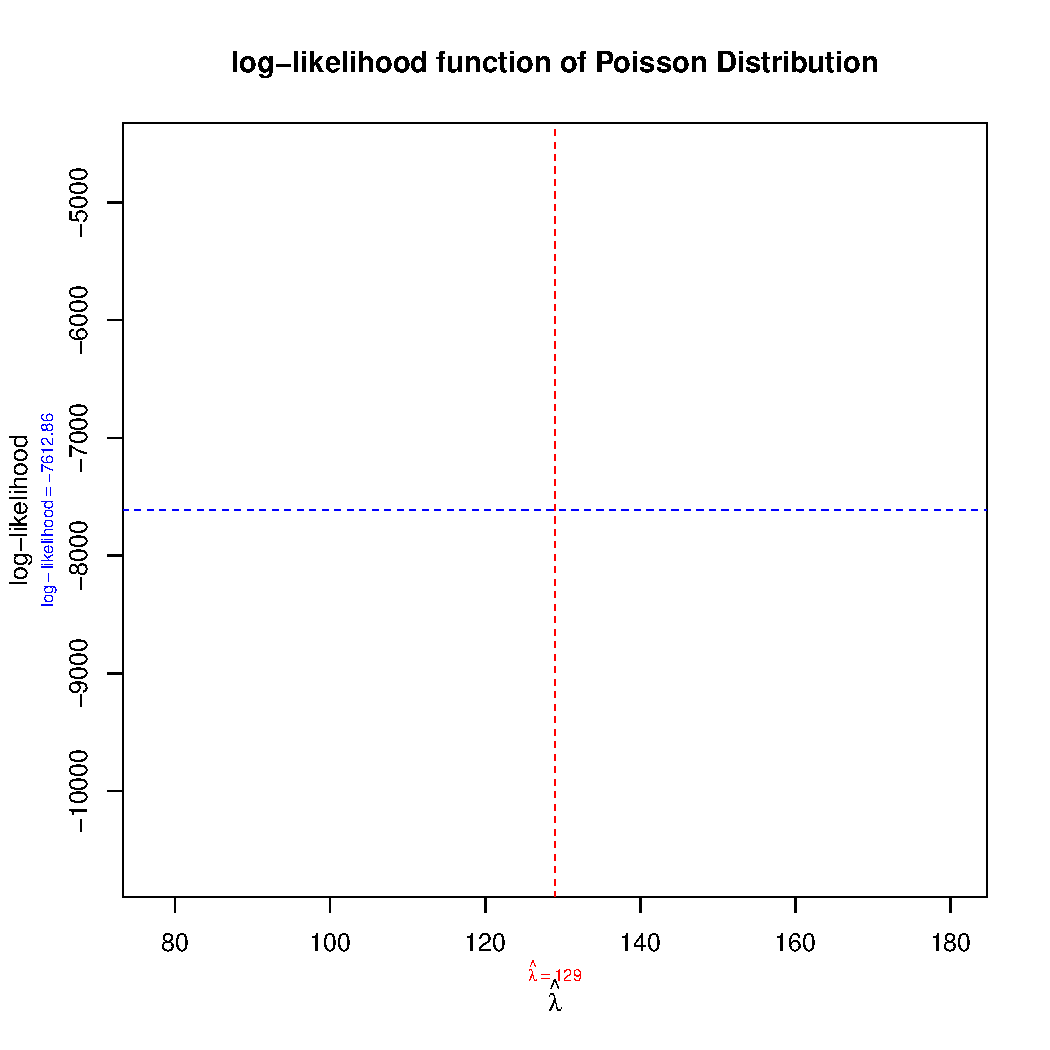
\includegraphics[width=\maxwidth]{figure/unnamed-chunk-3-1} \end{Schunk}

\section*{Exercise 4}
\noindent 1. Write down the null and the alternative hypotheses in mathematical form. \newline

{\bf Null hypothesis—} $H_0 : \rho = \rho_0$ \newline

{\bf Alternative hypothesis—} $H_1 : \rho \neq \rho_0$, \newline

where $\rho_0 = 0$\newline

\noindent2. Calculate the value of test statistic.
\begin{Schunk}
\begin{Sinput}
#set working directory
setwd(getwd())

#read data from file txt
body <- read.table(file = 'body-measurements.txt', header = T)

#get only body height of female
body.f.height <- body[body$sex == 'f', 'body.H']

#get only neck of female
body.f.neck <- body[body$sex == 'f', 'neck.C']

#na.omit will clean data that have NA value
body.f.height <- na.omit(body.f.height)
body.f.neck <- na.omit(body.f.neck)

#get length of the data
n.x <- length(body.f.height)
n.y <- length(body.f.neck)
n <- n.x <- n.y

#value of rho from null hypothesis
rho0 <- 0

#significant level
alpha <- 0.05

#calculate the estimate of rho using function cor()
#passing vector of body.f.height and body.f.neck
rho.est <- cor(body.f.height, body.f.neck, method = c("pearson", "kendall", "spearman"))

#calculate ZR using Fisher Z -variable
ZR <- 1/2 * log((1+ rho.est)/(1- rho.est))

#calculate the value of xi
xi <- 1/2 * log((1+ rho0)/(1-rho0))

#calculate the value of test statistics
zW <- sqrt(n -3)*(ZR - xi)
# round(zW, 5) => 1.39395
\end{Sinput}
\end{Schunk}
{\bf Result:} $zw = 1.39395$ \newline

\noindent 3. Calculate the critical region and make your decision.
\begin{Schunk}
\begin{Sinput}
#calculate critical value using qnorm for lower bound
z.CR.l <-qnorm(alpha/2, lower.tail = T)
# round(z.CR.l, 5) => -1.95996

#calculate critical value using qnorm for upper bound
z.CR.u <-qnorm(alpha/2, lower.tail = F)
# round(z.CR.u, 5) => 1.95996
\end{Sinput}
\end{Schunk}
{\bf Result:} $W = (-\infty, -1.95996) \cup (1.95996, \infty) $ \newline
The test statistic $zw = 1.39395$ does not belong to the critical region. Therefore we do not reject $H_0$. \newline

\noindent 4. Calculate the p-value and make your decision.
\begin{Schunk}
\begin{Sinput}
#calculate the p-value using test statistic value and pnorm()
p.val.zW <- 2 * (1 - pnorm(abs(zW)))
# round(p.val.zW, 5) => 0.16333
\end{Sinput}
\end{Schunk}
{\bf Result:} $p-value = 0.16333$ \newline
The p-value is {\bf 0.16333} which is greater than $\alpha = 0.05$. Therefore we do not reject $H_0$. \newline

\noindent 5. Plot the density of the distribution, that the test statistic follows, and visualise the p-value.
\begin{Schunk}
\begin{Sinput}
#create plot for bivariate distribution

#create data frame for body neck and height
df <- data.frame(body.f.neck, body.f.height)

#load library called MASS to use function kde2d
library(MASS)

#call function kde2d to generate density of body neck and height
body_density <- kde2d(df$body.f.neck, df$body.f.height, n=n)

#plot bivariate distribution
plot1 <- contour(body_density, xlab='Neck (mm)', ylab= 'Height (mm)', main='Density Distribution')

#add text showing p-value on top right of the plot
text(x = 355, y = 1820, labels = "p-value = 0.16333 ", xpd = NA, col = 'red')
\end{Sinput}

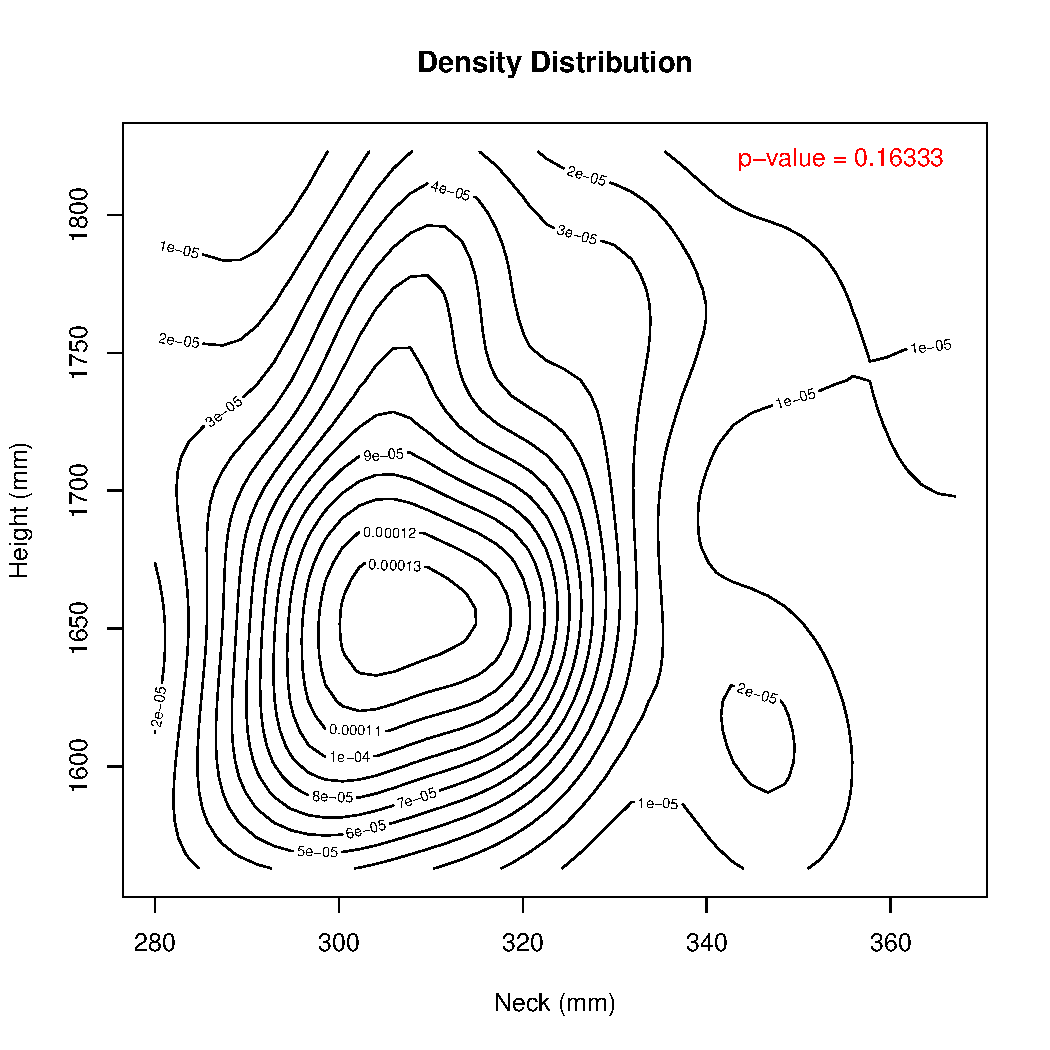
\includegraphics[width=\maxwidth]{figure/unnamed-chunk-7-1} \begin{Sinput}
#create another plot based on test statistics density distribution

#set sequence of test statistic from -3 to 3
zw.seq <- seq(-3,3, by = .1) 

#using dnorm to create density distribution
dvalues <- dnorm(zw.seq)

#plot the test statistic
plot2 <- plot(zw.seq, dvalues, type = 'l', xlab='Test statistic', ylab = 'Density', main = 'Test statistic distribution')

#add text under main title
text(x = 0, y = 0.42, labels = '(test statistic = 1.39395, alpha = 0.05)', col = 'black', xpd= NA)

#add vertical line for test statistic value and text
abline(v = zW, col = 'black', lty =2)
mtext(bquote(zw == .(round(zW, 2))), side = 1, line = 1.5,
      at = zW, cex = 0.7, col = 'black')

#add vertival line for lower bound critical region and text
abline(v = z.CR.l, col = 'red', lty =2)
mtext(bquote(alpha/2 == .(round(z.CR.l, 2))), side = 1, line = 2,
      at = z.CR.l, cex = 0.7, col = 'red')

#add vertical line for upper bound critical region and text
abline(v = z.CR.u, col = 'red', lty =2)
mtext(bquote(alpha/2 == .(round(z.CR.u, 2))), side = 1, line = 2,
      at = z.CR.u, cex = 0.7, col = 'red')

#add vertical line for p-value and text
abline(v = p.val.zW, col = 'blue', lty =2)
mtext(bquote(p-value == .(round(p.val.zW, 2))), side = 1, line = 2,
      at = p.val.zW, cex = 0.7, col = 'blue')
\end{Sinput}

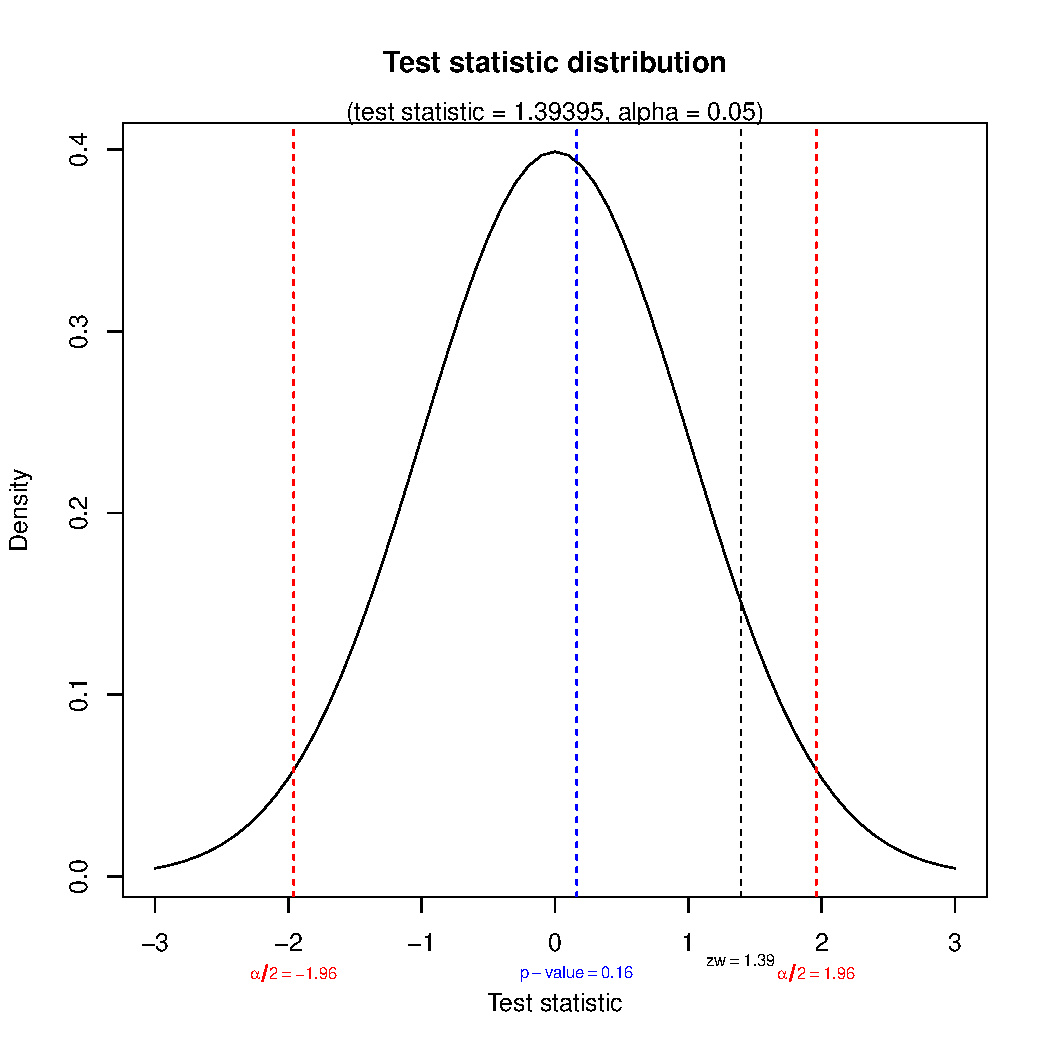
\includegraphics[width=\maxwidth]{figure/unnamed-chunk-7-2} \end{Schunk}

\noindent 6. Calculate the confidence interval for $\rho$ and make your decision.
\begin{Schunk}
\begin{Sinput}
#calculate the confidence interval Uaplha/2 = 1.95996 for lower bound
CI.zW.l <- tanh(ZR - 1.95996/sqrt(n-3))
# round(CI.zW.l, 5) => -0.08418

#calculate the confidence interval Uaplha/2 = 1.95996 for upper bound
CI.zW.u <- tanh(ZR + 1.95996/sqrt(n-3))
# round(CI.zW.u, 5) => 0.46209
\end{Sinput}
\end{Schunk}
{\bf Result:} $CI: (-0.08418, 0.46209)$ \newline
$\rho_0 = 0$ belongs to the value of $CI: (-0.08418, 0.46209)$. Therefore we do not reject $H_0$. \newline

\noindent 7. Interpret your conclusion. \newline

{\bf Statistical conclusion:} \newline
$H_0$ is not rejected on a significant level $\alpha = 0.05$, because (1) test statistics does not belong to critical region, (2) $\rho_0 = 0$ belongs to the confidence interval, and (3) p-value is greater than 0.05. \newline 

{\bf Verbal conclusion:} \newline
We are not rejecting null hypothesis that is stated there is no correlation between body height and neck circumference of females. \newline

\section*{Exercise 5}
\noindent 1. Write down the null and the alternative hypotheses in mathematical form. \newline

{\bf Null hypothesis—} $H_0: p_1 - p_2 = p_0$ \newline

{\bf Alternative hypothesis—} $H_1: p_1 - p_2 \neq p_0$, \newline

where $p_0 = 0$\newline

\noindent 2. Calculate the value of test statistic.
\begin{Schunk}
\begin{Sinput}
#setup first group data n1: number of product from group 1, x1: number of faulty product from group 1
n1 <- 200
x1 <- 32

#calculate the estimate probability of group 1
p1.est <- x1 / n1

#setup second group data n2: number of product from group 2, x2: number of faulty product from group 2
n2 <- 230
x2 <- 21

#calculate the estimate probability of group 2
p2.est <- x2 /n2

#calculate the estimate standard deviation
sd.est <- sqrt((p1.est*(1-p1.est))/n1 + (p2.est*(1-p2.est))/n2)

#value of p from null hypothesis
p0 <- 0

#significant level
alpha <- 0.05

#calculate the value of test statistics using Wald Test
zW.obs <- (p1.est - p2.est - p0)/sd.est
# round(zW.obs, 5) => 2.13765
\end{Sinput}
\end{Schunk}
{\bf Result:} $zw = 2.13765 $ \newline

\noindent 3. Calculate the critical region and make your decision.
\begin{Schunk}
\begin{Sinput}
#calculate the critical region for lower bound
z.CR.l <-qnorm(alpha/2, lower.tail = T)
# round(z.CR.l, 5) => -1.95996

#calculate the critical region for upper bound
z.CR.u <-qnorm(alpha/2, lower.tail = F)
# round(z.CR.u, 5) => 1.95996
\end{Sinput}
\end{Schunk}
{\bf Result:} $W = (-\infty, -1.95996) \cup (1.95996, \infty) $ \newline
The test statistic $zw = 2.13765$ belongs to the upper bound critical region. Therefore we reject $H_0$. \newline

\noindent 4. Calculate the p-value and make your decision.
\begin{Schunk}
\begin{Sinput}
#calculate the p-value using value of test statistic and pnorm()
p.val.zW <- 2 * (1 - pnorm(abs(zW.obs)))
# round(p.val.zW, 5) => 0.03255
\end{Sinput}
\end{Schunk}
{\bf Result:} $p-value = 0.03255$ \newline
The p-value is {\bf 0.03255} which is smaller than $\alpha = 0.05$. Therefore we reject $H_0$. \newline

\noindent 5. Calculate the confidence interval and make your decision.
\begin{Schunk}
\begin{Sinput}
#calculate the confidence interval for lower bound Ualpha/2 = 1.95996
CI.zW.l <- p1.est - p2.est - (1.95996 * sd.est)
# round(CI.zW.l, 5) => 0.00571

#calculate the confidence interval for upper bound Ualpha/2 = 1.95996
CI.zW.u <- p1.est - p2.est + (1.95996 * sd.est)
# round(CI.zW.u, 5) => 0.13168
\end{Sinput}
\end{Schunk}
{\bf Result:} $CI: (0.00571, 0.13168)$ \newline
$p_0 = 0$ does not belong to the value of $CI: (0.00571, 0.13168)$. Therefore we reject $H_0$. \newline

\noindent 6. Interpret your conclusion. \newline

{\bf Statistical conclusion:} \newline
$H_0$ is rejected on a significant level $\alpha = 0.05$, because (1) test statistics belongs to critical region, (2) $p_0 = 0$ does not belong to the confidence interval, and (3) p-value is less than 0.05. \newline 

{\bf Verbal conclusion:} \newline
We are rejecting null hypothesis that the probability of getting a faulty product are the same in both factories.

\end{document}
